\documentclass[12pt]{article}

\usepackage{sbc-template}
\usepackage[utf8]{inputenc}
\usepackage[brazil]{babel}% este é para o texto

\usepackage{graphicx,url}

     
\sloppy

\title{Mineração de Dados Distribuída Aplicada à Detecção de Desvios Comportamentais no Contexto da Internet das Coisas}

\author{Ricardo de Azevedo Brandão\inst{1} }


\address{Instituto Militar de Engenharia
  (IME)\\
  Praça General Tibúrcio, 80 -- Rio de Janeiro -- RJ -- Brasil
  \email{rbrandao@ime.eb.br}
}

\begin{document} 

\maketitle

\begin{abstract}
Mussum Ipsum, cacilds vidis litro abertis. Mé faiz elementum girarzis, nisi eros vermeio. Manduma pindureta quium dia nois paga. Ta deprimidis, eu conheço uma cachacis que pode alegrar sua vidis.” Mauris nec dolor in eros commodo tempor. Aenean aliquam molestie leo, vitae iaculis nisl.

Per aumento de cachacis, eu reclamis. Mais vale um bebadis conhecidiss, que um alcoolatra anonimiss. Quem num gosta di mé, boa gente num é. Suco de cevadiss deixa as pessoas mais interessantiss. 
\end{abstract}
     
\begin{resumo} 
    A internet das coisas é um termo utilizado para representar coisas (sensores e atuadores) conectadas à Internet. Ao longo dos últimos anos a quantidade de dispositivos têm crescido exponencialmente bem como a quantidade de dados gerados pelas interações desses equipamentos. Nesse contexto a mineração de dados tem enfrentado um grande desafio devido principalmente ao caráter dinâmico da topologia de uma rede de Internet das Coisas. As técnicas tradicionais de mineração de dados são centralizadas e considera uma condição estática do conjunto de dados. Esse artigo tem como objetivo apresentar estudos relativos à mineração de dados descentralizada e a detecção de desvios de padrões.
\end{resumo}

\section{Introdução}

O avanço tecnológico que possibilitou a redução de tamanho de processadores, aliada ao aumento de capacidade de processamento abriu caminho para uma proliferação de equipamentos com os mais diversos propósitos. Havia uma tendência natural que esses dispositivos se conectassem à internet a fim de compartilhar os dados coletados com nós geograficamente dispersos e permitir que usuários pudessem enviar comandos para esses objetos de forma remota.

Ao longo do tempo, mesmo que não tenhamos dado conta, essas "coisas" \footnote{Ao longo desse artigo serão utilizaos os termos dispositivos, objetos e coisas para representar qualquer equipamento conectado à internet} começaram a fazer parte de nossas vidas alterando significativamente a forma como os indivíduos se relacionam.

Para representar essa extensão da internet que rompeu os limites das redes de computadores, participando de forma pervasiva no dia a dia das pessoas, foi cunhado o termo Internet das Coisas.

De acordo com \cite{000-000} a Internet das coisas nasceu com o propósito ousado de conectar todas as coisas do mundo na internet.

A indústria e a academia têm trabalhado na construções de ambientes compostos por sistemas inteligentes em diversas áreas como casas inteligentes, transporte, logística e saúde \cite{000-000}.

Outra linha de pesquisa tem aprofundado a questão da arquitetura dos dispositivos como em \cite{000-006} no qual é proposta uma análise abrangente do estado da arte da Internet das coisas abordando uma proposta de desenho de arquitetura de três camadas: (i) Tecnológica, (ii) Acesso (iii) Internet, (iv) \textit{Middleware} e (v) Aplicação. Já em \cite{000-003} o autor aprofunda o assunto com foco no desenvolvimento para dispositos de Internet das Coisas, detalhando os quesitos técnicos da arquitetura.

Porém, uma das mais importantes questões que tem surgido é como converter os dados gerados ou capturados pela Internet das Coisas em conhecimento \cite{000-000}. Então diversas técnicas de KDD (\textit{Knowledge Discovery in Databases}) e Mineração de dados têm sido aplicadas para analisar os dados com o objetivo de melhorar os serviços providos pelos ambientes formados por esses dispositivos.

Diversos trabalhos apresentam algoritmos de mineração de dados em Internet das Coisas:  \cite{000-014} aborda a mineração em rede de sensores distribuídos,  \cite{000-015} em dispositivos RFID, \cite{000-056} apresenta algoritmos de clusterização para rede de sensores em fio e em \cite{003-000} são propostos quatro métodos diferentes de mineração de dados em Internet das Coisas.

Os dados na Internet das Coisas podem ser classificados em dados sobre as coisas, como estado, localização, etc e dados gerados pelas coisas. Esses últimos contém dados representativos das interações entre: (i) coisas, (ii) humanos e coisas e (iii) entre humanos \cite{000-018}. Assim, ao utilizar técnicas de detecção de padrões é possível identificar o comportamento das coisas e dos humanos cujos dados são coletados pelos dispositivos, que por sua vez possibilitam identificar desvios comportamentais dos objetos e pessoas monitorados. 

Técnicas de detecção de comportamento são utilizadas em identificação de padrões de atividade em ambientes inteligentes: \cite{000-062}, \cite{008-000}, \cite{009-000}, \cite{009-038}, \cite{010-000}, análise de consumidores, \cite{000-111} e \cite{000-123}, Detecção de Intrusos \cite{004-000}.

Esse artigo tem como objetivo apresentar um resumo dos trabalhos apresentados na área de Mineração de Dados Distribuída no Contexto de Internet das Coisas. Na Seção \ref{sec:dadosIoT} apresenta um breve resumo do conceito de Internet das Coisas e sobre os dados gerados pelos dispositivos. As técnicas de Mineração de Dados são tratadas na Seção \ref{sec:MDIoT} com detalhamento sobre Mineração de Dados distribuída na Seção \ref{MDD}. Na seção \ref{sec:DetecDesvios} são tratadas as técnicas de Detecção de Padrões e dos desvios de comportamento. A conclusão, problemas em aberto e próximos trabalhos são tratados na Seção  \ref{sec:Conclusao}.

\section{Dados gerados pela Internet das Coisas} \label{sec:dadosIoT}

Mussum Ipsum, cacilds vidis litro abertis. Quem num gosta di mé, boa gente num é. Todo mundo vê os porris que eu tomo, mas ninguém vê os tombis que eu levo! Manduma pindureta quium dia nois paga. Si num tem leite então bota uma pinga aí cumpadi!

Viva Forevis aptent taciti sociosqu ad litora torquent Interessantiss quisso pudia ce receita de bolis, mais bolis eu num gostis. Delegadis gente finis, bibendum egestas augue arcu ut est. Leite de capivaris, leite de mula manquis.

\section{Mineração de Dados na Internet das Coisas} \label{sec:MDIoT}

Mussum Ipsum, cacilds vidis litro abertis. Todo mundo vê os porris que eu tomo, mas ninguém vê os tombis que eu levo! Suco de cevadiss, é um leite divinis, qui tem lupuliz, matis, aguis e fermentis. Ta deprimidis, eu conheço uma cachacis que pode alegrar sua vidis.” Vehicula non. Ut sed ex eros. Vivamus sit amet nibh non tellus tristique interdum.

Não sou faixa preta cumpadi, sou preto inteiris, inteiris. Quem num gosti di mum que vai caçá sua turmis! Mais vale um bebadis conhecidiss, que um alcoolatra anonimiss. Admodum accumsan disputationi eu sit. Vide electram sadipscing et per. 

\section{Mineração de Dados Distribuída} \label{MDD}

Mussum Ipsum, cacilds vidis litro abertis. Mauris nec dolor in eros commodo tempor. Aenean aliquam molestie leo, vitae iaculis nisl. Casamentiss faiz malandris se pirulitá. Atirei o pau no gatis, per gatis num morreus. Cevadis im ampola pa arma uma pindureta.

Admodum accumsan disputationi eu sit. Vide electram sadipscing et per. Si num tem leite então bota uma pinga aí cumpadi! Ta deprimidis, eu conheço uma cachacis que pode alegrar sua vidis.” Vehicula non. Ut sed ex eros. Vivamus sit amet nibh non tellus tristique interdum.


\subsection{Subsections}

The subsection titles must be in boldface, 12pt, flush left.

\section{Figures and Captions}\label{sec:figs}

Figure and table captions should be centered if less than one line
(Figure~\ref{fig:exampleFig1}), otherwise justified and indented by 0.8cm on
both margins, as shown in Figure~\ref{fig:exampleFig2}. The caption font must
be Helvetica, 10 point, boldface, with 6 points of space before and after each
caption.

\begin{figure}[ht]
\centering
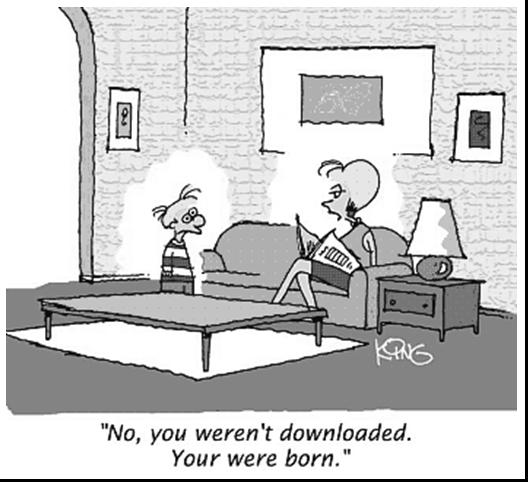
\includegraphics[width=.5\textwidth]{fig1.jpg}
\caption{A typical figure}
\label{fig:exampleFig1}
\end{figure}

\begin{figure}[ht]
\centering
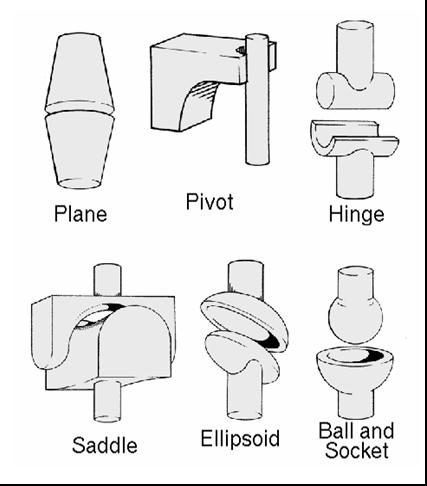
\includegraphics[width=.3\textwidth]{fig2.jpg}
\caption{This figure is an example of a figure caption taking more than one
  line and justified considering margins mentioned in Section~\ref{sec:figs}.}
\label{fig:exampleFig2}
\end{figure}

In tables, try to avoid the use of colored or shaded backgrounds, and avoid
thick, doubled, or unnecessary framing lines. When reporting empirical data,
do not use more decimal digits than warranted by their precision and
reproducibility. Table caption must be placed before the table (see Table 1)
and the font used must also be Helvetica, 10 point, boldface, with 6 points of
space before and after each caption.

\begin{table}[ht]
\centering
\caption{Variables to be considered on the evaluation of interaction
  techniques}
\label{tab:exTable1}
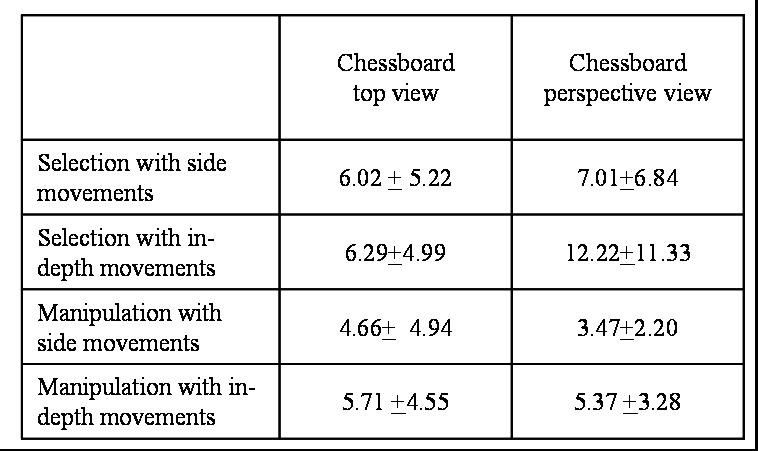
\includegraphics[width=.7\textwidth]{table.jpg}
\end{table}

\section{Detecção de desvios} \label{sec:DetecDesvios}

Mussum Ipsum, cacilds vidis litro abertis. Casamentiss faiz malandris se pirulitá. Detraxit consequat et quo num tendi nada. Cevadis im ampola pa arma uma pindureta. Nec orci ornare consequat. Praesent lacinia ultrices consectetur. Sed non ipsum felis.

Copo furadis é disculpa de bebadis, arcu quam euismod magna. Mé faiz elementum girarzis, nisi eros vermeio. A ordem dos tratores não altera o pão duris Delegadis gente finis, bibendum egestas augue arcu ut est.


\section{Conclusão} \label{sec:Conclusao}

Mussum Ipsum, cacilds vidis litro abertis. Casamentiss faiz malandris se pirulitá. Detraxit consequat et quo num tendi nada. Cevadis im ampola pa arma uma pindureta. Nec orci ornare consequat. Praesent lacinia ultrices consectetur. Sed non ipsum felis.

Copo furadis é disculpa de bebadis, arcu quam euismod magna. Mé faiz elementum girarzis, nisi eros vermeio. A ordem dos tratores não altera o pão duris Delegadis gente finis, bibendum egestas augue arcu ut est.



\section{References}

Bibliographic references must be unambiguous and uniform.  We recommend giving
the author names references in brackets, e.g..

The references must be listed using 12 point font size, with 6 points of space
before each reference. The first line of each reference should not be
indented, while the subsequent should be indented by 0.5 cm.

\bibliographystyle{sbc}
\bibliography{sbc-template}

\end{document}
